\chapter{Computational Challenges prior to Simulating}

\section{Converting Secular Frequencies to Electric Fields}\label{sec:comp/freqs2aq}

TODO: \cite{AkermanThesis}

\section{Coulomb Energy Effect on Temperature}\label{sec:comp/coulomb}

We wish to study sympathetic cooling starting from a thermodynamically stable state. This helps reduce the random effects of thermodynamic instabilities, which can be computationally expensive to ignore, although in experiment, these instabilities might not affect much the cooling. This raises a few important questions: How significant is the Coulomb potential energy in the Boltzmann ensemble? Should it be considered when initiating the positions and velocities of the ions?

Under the secular approximation, and when ignoring the Coulomb potential, the Maxwell-Boltzmann partition function dictates the probability of finding an ion in a position $\mathbf{x}$ to be:

\begin{equation}
	\prod_{i=1}^3 \sqrt{\frac{k_i}{2\pi K_\text{B} T}} \exp\left(\frac{-k_i x_i^2}{2 K_\text{B} T}\right)
	\label{eq:position-probability}
\end{equation}

Where $k_i$ is the spring-like coefficients of the harmonic trap. This distributions couples naturally density and temperature. We are interested in measuring the Coulomb energy per particle (denoted as $E_c/N$) as a function of the parameters of the distribution function above. Since the real temperature is affected by the Coulomb energy, we'd not use the symbol $T$ in the following usages of expression \ref{eq:position-probability}, but rather $\tau$. The parameters that can affect $E_c/N$ are: $\{k_i\}$, $\tau$, and most importantly the number of ions $N$.

The relation of $E_c/N$ to it's parameters is not analytical, yet we still expect a smooth behavior if we'd average over enough randomness. In figure \ref{fig:coulomb_energy} we can see that (expectedly), dense and cold ion clouds produce a higher Coulomb energy, that even exceeds $\tau$.

\begin{figure}
	\begin{center}
		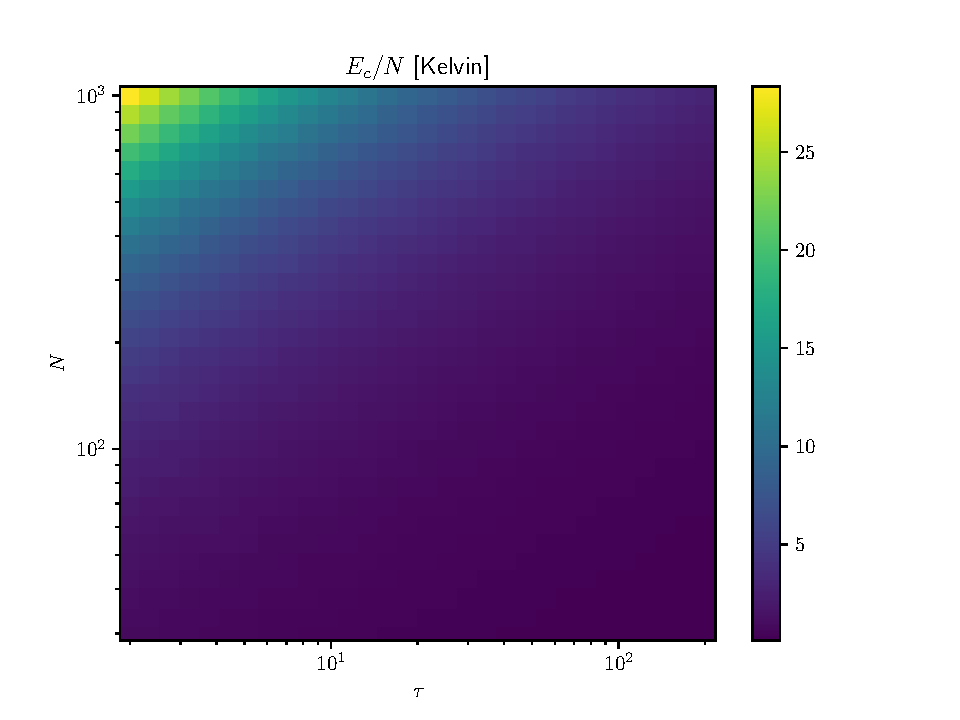
\includegraphics[width=0.95\textwidth]{graphics/coulomb_energy_example@coulomb_energy.pdf}
	\end{center}
	\caption{Example dependence of $E_c/N$ to $N$ and $\tau$ for a trap of \ce{Yb^+} with secular frequencies of $(8.5, 8.5, 1.5) \mathrm{kHz}$, in the range of $\tau\in[2, 200]\mathrm{K}$.}\label{fig:coulomb_energy}
\end{figure}

To produce this smooth color-mesh, we distributed the ions in space multiple times per $(\tau,N)$ point, until the relative standard deviation of all $E_c/N$ results in that point was lower then $0.12$, with a minimum of 5 distributions (also termed 'iterations'). Statistical results of figure \ref{fig:coulomb_energy} are available in the appendix.
% TODO: Add \ref to the above and

Naturally, the value of the highest Coulomb energy found escalates with the trap's tightness, as can be seen in figure \ref{fig:coulomb_energy_f_z}.

\begin{figure}
	\begin{center}
		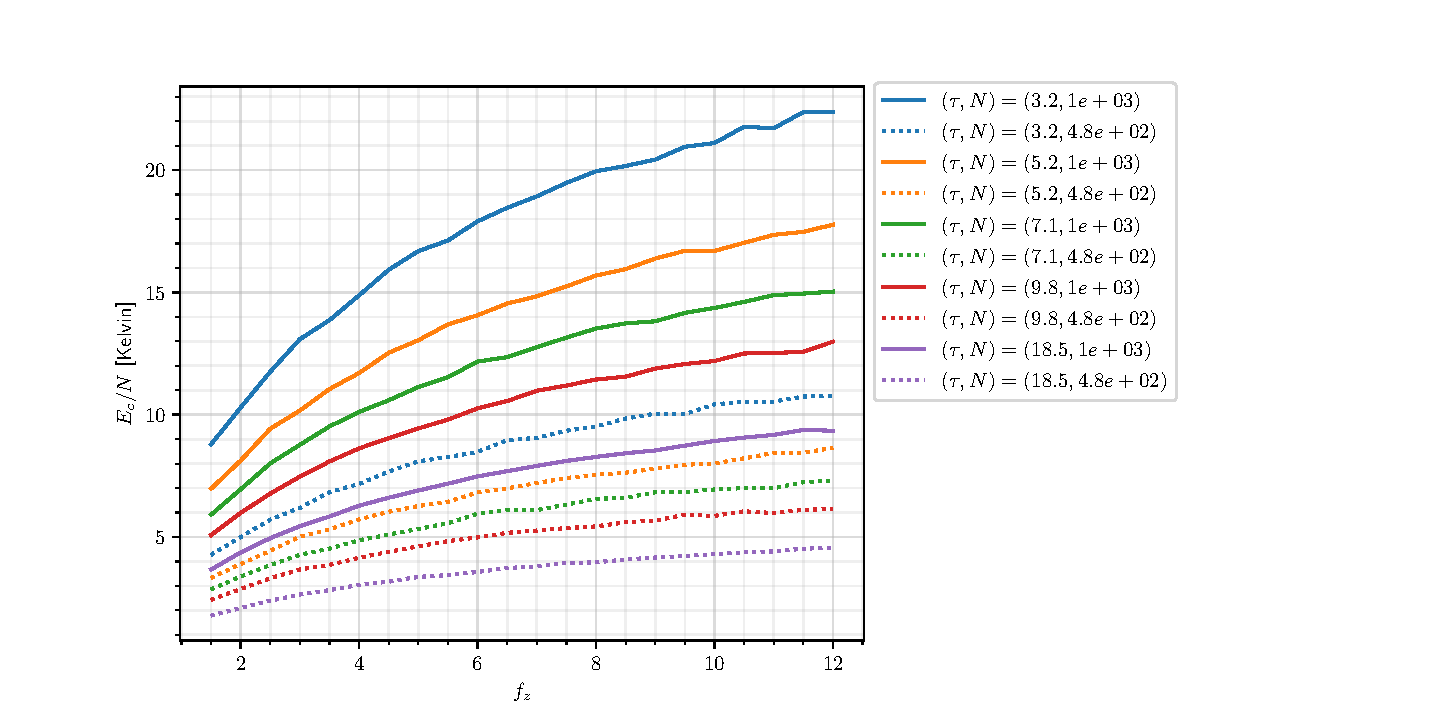
\includegraphics[width=1.2\textwidth]{graphics/coulomb_energy_f_z.pdf}
	\end{center}
	\caption{The dependence of $E_c/N$ upon the z secular frequency, for a few specific $(\tau,N)$ pairs, and $f_x = f_y = 8.5\mathrm{kHz}$.}\label{fig:coulomb_energy_f_z}
\end{figure}

To \textbf{summarize}, the Coulomb energy is not negligible for dense \& cold distributions. Our ability to initiate a distribution of ions in a thermodynamically stable set of positions is limited by the effects of strong Coulomb energy, and by the tightness of our trap. To avoid too strong Coulomb energy effects, we thereby avoid distributing ions in $T < 5\mathrm{K}$.\footnote{During the research period I tried to construct an algorithm that would find a $\tau$ for a given $N$ and a given secular frequencies, such that the system will be more thermodynamically stable initially. When this algorithm was used for a single ion species it was slightly effective. However when 2 ion species were used, (with different masses and different $\{k_i\}$ - see section \ref{sec:comp/freqs2aq}), accommodating the algorithm for that case has proved to be too complex, and too slow.} More importantly, we expect time dependent temperature measurements to be offset from the initial temperature $T_i$ on the order of magnitude of the Coulomb energy. Since we also wish to start cooling when the system is thermodynamically stable, the Coulomb energy offset requires us to wait for a few $\mathrm{ms}$, before beginning cooling, as can also be seen from the oscillations in figure. % TODO: \ref{fig:}

\section{RF division Finesse, Stability \& Convergence}\label{sec:comp/convergence}

% TODO: Explain how RF division is critical.
